% !TeX spellcheck = en_GB
%PREAMBLE - SETTING FOR CREATING A REPORT
\documentclass[12pt,a4paper,titlepage]{article}
\usepackage[utf8]{inputenc}
\usepackage{graphicx}
\usepackage{float}
\usepackage{amsmath}
\usepackage{amsfonts}
\usepackage{amssymb}
\usepackage{courier}
\usepackage{enumitem}

\usepackage{caption}
\usepackage{subcaption}
\usepackage{listings}
\usepackage{color} %red, green, blue, yellow, cyan, magenta, black, white
\definecolor{mygreen}{RGB}{28,172,0} % color values Red, Green, Blue
\definecolor{mylilas}{RGB}{170,55,241}

\lstset{language=Matlab,%
	basicstyle=\footnotesize\ttfamily,
	breaklines=true,%
	morekeywords={matlab2tikz},
	keywordstyle=\color{blue},%
	morekeywords=[2]{1}, keywordstyle=[2]{\color{black}},
	identifierstyle=\color{black},%
	stringstyle=\color{mylilas},
	commentstyle=\color{mygreen},%
	showstringspaces=false,%without this there will be a symbol in the places where there is a space
	numbers=left,%
	numberstyle={\tiny \color{black}},% size of the numbers
	numbersep=9pt, % this defines how far the numbers are from the text
	emph=[1]{for,end,break},emphstyle=[1]\color{red}, %some words to emphasise
	%emph=[2]{word1,word2}, emphstyle=[2]{style},    
}


\title{\Huge Face Recognition using PCA \\ \Large Applied Mathematics Homework}

\author{Report by: \\ Savinien Bonheur and Albert Clerigues}

\date {January 6, 2016}
%SETTINGS END

\begin{document}

%CREATE TITLE IN THE FIRST PAGE
\maketitle

%START A NEW PAGE
\pagebreak

\section{Data Normalization}

The first step to classify faces based on pixel information is to make sure the training samples and the ones to classify are as similar and standard as possible. For this matter we will make two normalization steps: 

\begin{enumerate}
	\item Light correction, to compensate for non-uniform lightning of pixels in the image and between the samples.
	\item Feature mapping, to make sure the pixel data is aligned and corresponds to each feature.
\end{enumerate}

\subsection{Light Correction}
To perform light correction we make a simplified light intensity image based on approximating a linear model to fit the original image light intensity. Once we have this simplified model we subtract it from the original model to get a light corrected image. The last step is to normalize the contrast range to the [0-255]  uint8 range and round.

\begin{figure}[H]
	\centering
	\begin{subfigure}{0.3\columnwidth}
		\centering
		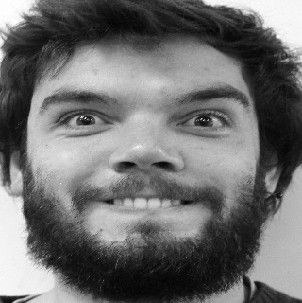
\includegraphics[width=\textwidth]{lightCorrection1.jpg}
		\caption{Original}
	\end{subfigure}
	\quad
	\begin{subfigure}{0.3\textwidth}
		\centering
		
\includegraphics[width=\textwidth]{lightCorrection2.jpg}
		\caption{Fitted model}
	\end{subfigure}	
	\quad
	\begin{subfigure}{0.3\textwidth}
		\centering
		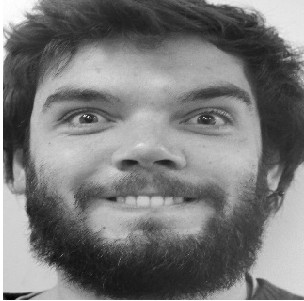
\includegraphics[width=\textwidth]{lightCorrection3.jpg}
		\caption{Result}
	\end{subfigure}
	\caption{Example of application of light correction}
\end{figure}

It can be seen that the right of the original face was in shadow and darker than the other, after the correction both sides of the face have approximately the same average intensity.

\subsection{Normalized Feature Mapping}

In order to have the same physical area of the face coincide with each feature pixel in all images we have to transform the image. For this matter we will select key face features and approximate a transform that maps the original image face with the standard face model. 

The output image must be of dimension 64x64 and have the facial features mapped according to the reference face:

\begin{figure}[H]
	\centering
	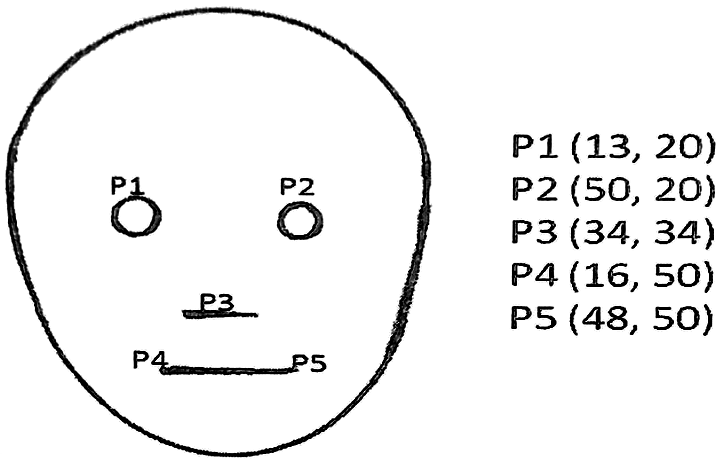
\includegraphics[width=0.4\textwidth]{facialFeatures}
	\caption{Location of the five facial features in the reference face}
\end{figure}

The process of finding such transformation will be implemented using an iterative algorithm that uses SVD to find the Least Linear Squares approximation for the transform. It is not possible to find it by directly solving the linear system since it is overdetermined, having 10 equations and 6 unknowns.

\begin{figure}[H]
	\centering
	\begin{subfigure}{0.3\columnwidth}
		\centering
		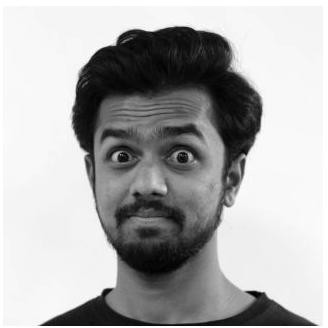
\includegraphics[width=\textwidth]{mapping1.jpg}
		\caption{Original Nayeem}
	\end{subfigure}
	\quad
	\begin{subfigure}{0.3\textwidth}
		\centering
		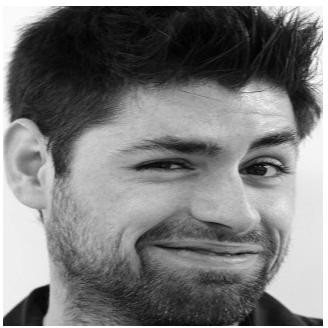
\includegraphics[width=\textwidth]{mapping3.jpg}
		\caption{Original Dani}
	\end{subfigure}	
	\quad
	\begin{subfigure}{0.3\columnwidth}
		\centering
		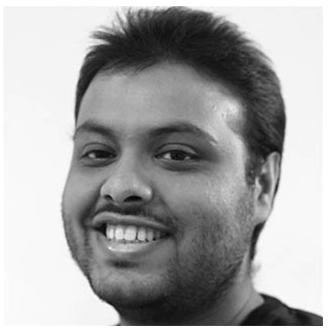
\includegraphics[width=\textwidth]{mapping5.jpg}
		\caption{Original Hassan}
	\end{subfigure}
	\\
	\begin{subfigure}{0.3\textwidth}
		\centering
		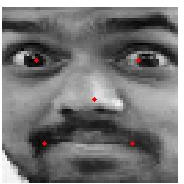
\includegraphics[width=\textwidth]{mapping2.jpg}
		\caption{Transformed Nayee}
	\end{subfigure}	
	\quad
	\begin{subfigure}{0.3\columnwidth}
		\centering
		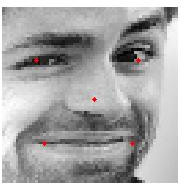
\includegraphics[width=\textwidth]{mapping4.jpg}
		\caption{Transformed Dani}
	\end{subfigure}
	\quad
	\begin{subfigure}{0.3\textwidth}
		\centering
		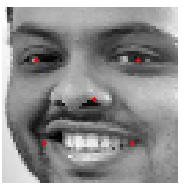
\includegraphics[width=\textwidth]{mapping6.jpg}
		\caption{Transformed Hassan}
	\end{subfigure}	
	\caption{Example of feature mapping, standard feature locations are marked in red in the transformed images}
\end{figure}


\section{Face Recognition}

\subsection{Dimensionality Reduction with PCA}

The normalized images contain 4096 pixels which corresponds to 4096 features to compare for the Nearest Neighbour search. We can simplify this problem with PCA reducing the number of features while being less sensitive to noise. By projecting the image into a meaningful base we can get rid of the less distinctive components and use the coefficients that convey more distinctive information for matching the faces.

For this, the images are projected into a base computed with the training data using PCA with \emph{getPCABase(TrainImages)}. The test and train images are projected into the same base and the resulting coefficients are stored.

The ideal thing to do would be projecting only the first $c$ components we needed (for face-recognition $c \approx$ 100) to save memory later. However, the dimensionality reduction is performed at the time of classification, since we value more being able to change the number of components for classification at any given time than saving some memory by projecting only on the desired number of components. For a final application based on this concept, a number of components $c$ would be fixed and the images projected on the first $c$ eigenvectors of the base before storing.


\section{The Implementation}
The code provided is divided in three main sections being database loading and handling, GUI, and utility functions. 


\paragraph{}Database loading and handling includes the next functions:
\vspace{-0.5em}
\begin{itemize}[itemsep=0.05em]
	\item \texttt{loadDataFolder.m} - Loads the images and features from a given directory.
	\item \texttt{prepareTrainAndTest.m} - Normalizes the Train and Test data sets and gets the PCA projection of both.
\end{itemize}

\paragraph{}The program GUI is implemented and launched in:
\vspace{-0.5em}
\begin{itemize}[itemsep=0.05em]
	\item \texttt{a\_launchPCFace.m} - Loads the Train and Test data sets and launches the GUI.
 	\item \texttt{GUI.m} - Handles all the GUI operation.
\end{itemize}

\paragraph{}Finally, the functionality of the face recognition is implemented with:
\vspace{-0.5em}
\begin{itemize}[itemsep=0.05em]
    \item \texttt{applyImageTransform.m} - Applies the given transform to the image through inverse mapping.
	\item \texttt{computeLMStransform.m} - Computes the approximated transform to map the feature vector to the standard face.
	\item \texttt{light\_correction.m} - Applies the light correction algorithm to the given image.
	\item \texttt{normalizeImages.m} - Performs all the previous steps to a set of images and outputs the normalized versions.
	
	\item \texttt{getPCABase.m} - Obtains the PCA base of eigenvectors for a given set of images.
	\item \texttt{projectPCABase.m} - Projects a set of images into the given base and returns the coefficients
	\item \texttt{matchNN.m} - Performs Nearest Neighbour classification based on the given Training set and the Test image.
	
	\item \texttt{recogniseFace.m} - Selects only the first $k$ components of the given data sets and uses matchNN to get the nearest neighbour.
\end{itemize}


\subsection{User guide}
	To run the program:
	\begin{enumerate}
		\item Run the script "a\_launchPCFace.m" which will load the data sets and launch the GUI.
		\item In the GUI, press the button named "Train" to execute the normalization and projection of the loaded data sets.
		\item Scroll the top right list of test images and select one which you would like to recognise. 
		
		After that press the "Find" button below it. The lower right list should update with a list of the names of the most probable names along with the certainty score percentage (relative to the smallest and biggest distances).
	\end{enumerate}
	 
	
\section{Results and Conclusions}

 \subsection{Results}
\begin{figure}[H]
	\centering
	\begin{subfigure}{0.48\columnwidth}
		\centering
		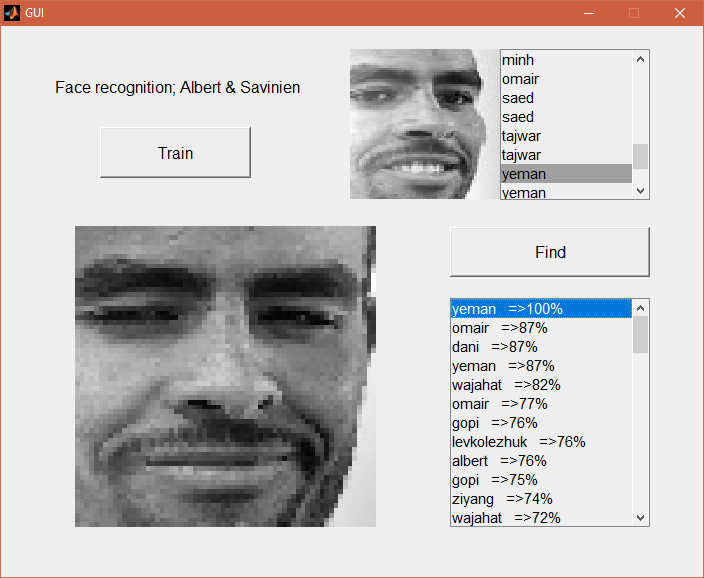
\includegraphics[width=\textwidth]{gui1}
		\caption{Yeman 1st match}
	\end{subfigure}
	\quad
	\begin{subfigure}{0.48\textwidth}
		\centering
		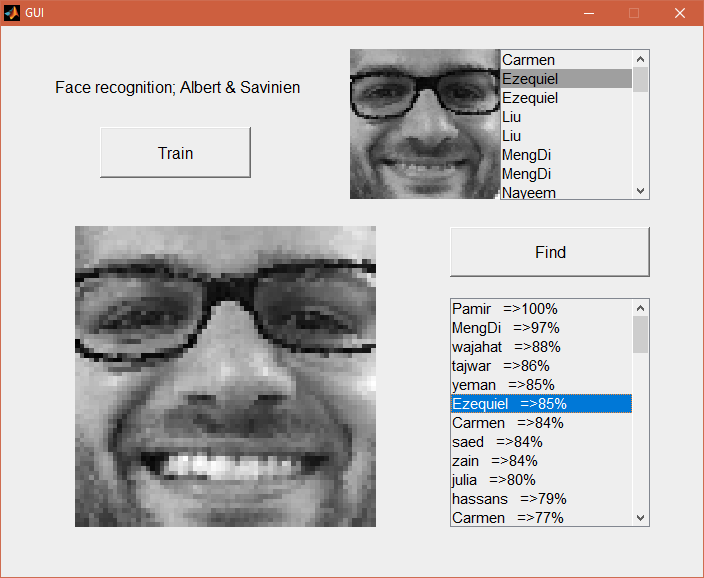
\includegraphics[width=\textwidth]{gui2}
		\caption{Eze 5th match}
	\end{subfigure}	
\\
	\vspace{1em}
	\begin{subfigure}{0.48\textwidth}
		\centering
		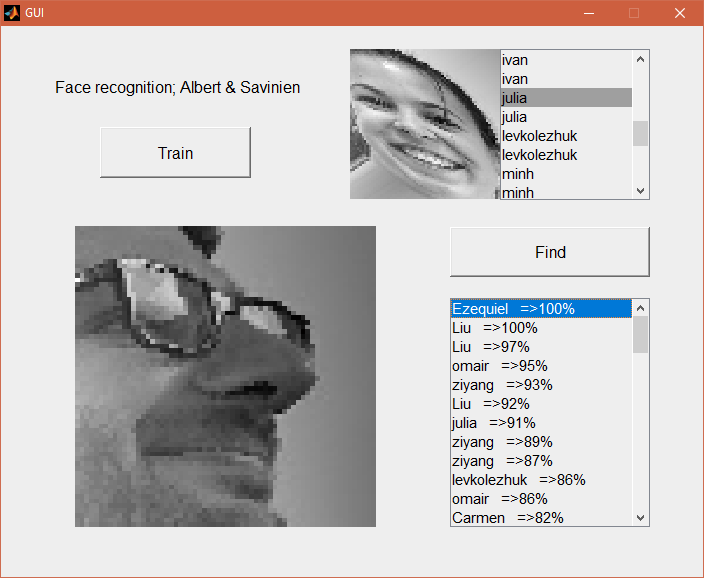
\includegraphics[width=\textwidth]{gui3}
		\caption{Julia bad features}
	\end{subfigure}	
	\quad
	\begin{subfigure}{0.48\columnwidth}
		\centering
		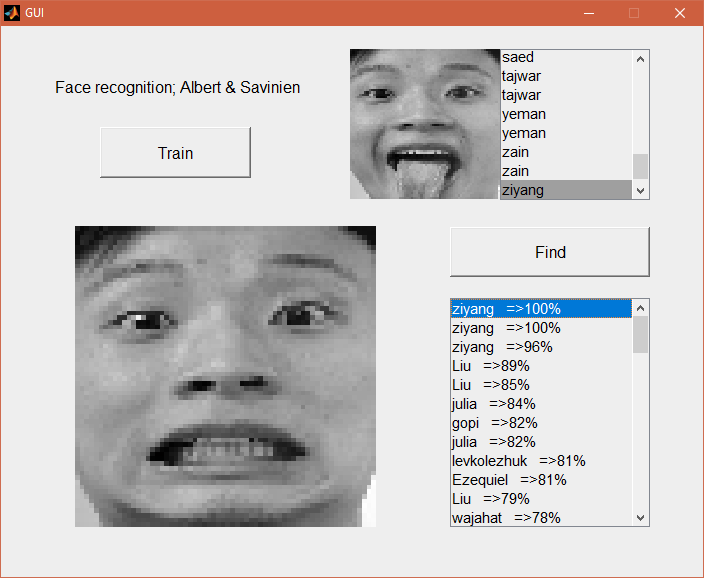
\includegraphics[width=\textwidth]{gui4}
		\caption{Ziyang 1st match}
	\end{subfigure}
	\caption{Example of different classifications with the developed program.}
\end{figure}


The program successfully recognises a big percentage of faces in the test data set. We measured the accuracy of the classifier according with the formula:

\begin{equation}
	\text{Accuracy (\%)} = \left(1 - \dfrac{\epsilon_k}{N_{\text{test images}}}\right) \cdot 100
\end{equation}

Where $\epsilon_k$ is the number of classifications that didn't provide the right label in the first k positions. We also check how the precision evolves according to the number of components used for classification.

\begin{figure}[H]
	\centering
	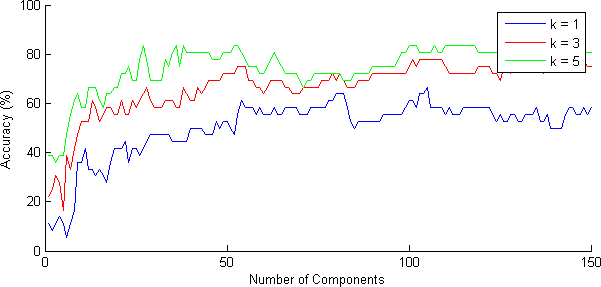
\includegraphics[width=1.0\textwidth]{accuracy}
	\caption{Recognition accuracy (\%) for different  $\epsilon_k$ and number of components}
\end{figure}

With enough number of components (c \textgreater~60) the classifier has an accuracy of around 50\% for first match on the test dataset, getting up to 65\% for first three matches. The result is satisfactory although it is far from optimal, the main weaknesses of this classifier are its dependency on the quality of data such as the right tagging of features and the similarity of face expression of the image to be recognised with any of the training set.

\subsection{Conclusions}
Classification of image content using PCA is tricky since you need normalized data such that all the features are uniform throughout the samples (e.g. the pixels in each image must correspond to the same physical location, the lightning conditions similar, good sampling of many angles...). 

On the other side, we have also seen how much the problem is reduced from 4096 original features to 60, a reduction to 1.5\% of the original size, which translates in less memory to store the databases and less computation time for classification.


%\begin{figure}[H]
%	\centering
%	\begin{subfigure}{0.3\columnwidth}
%		\centering
%		\includegraphics[width=\textwidth]{lms0deg}
%		\caption{Polarizer 0$º$}
%	\end{subfigure}
%	\quad
%	\begin{subfigure}{0.3\textwidth}
%		\centering
%		\includegraphics[width=\textwidth]{lms45deg}
%		\caption{Polarizer 45$º$}
%	\end{subfigure}	
%	\quad
%	\begin{subfigure}{0.3\textwidth}
%		\centering
%		\includegraphics[width=\textwidth]{lms90deg}
%		\caption{Polarizer 90$º$}
%	\end{subfigure}
%\end{figure}
%
%
%\begin{lstlisting}
%Im0 = im2double(imread('lms0deg.png'));
%Im45 = im2double(imread('lms45deg.png'));
%Im90 = im2double(imread('lms90deg.png'));
%
%ColorImage = hsv2rgb(ColorImage);
%\end{lstlisting}
%
%\begin{figure}[H]
%	\centering
%	\includegraphics[width=0.8\textwidth]{hsvimage}
%	\caption{HSV mapped image of polarization parameters}
%\end{figure}

\end{document}
